\chapter{Classification methods }
In previous chapter, we introduce a method to remove the unexpected object. In this chapter, we will propose a method to obtain the features what we are interested in and the method to detect the landmarks on the insect. This method was proposed by Palaniswamy$^{\cite{palaniswamy2010automatic}}$.
\section{Preprocessing image and feature extraction}
Feature extraction stage is duration that we extract essential information from the digital images and retaining only these features that we are interested in. To obtain the good result, before extracting the features in the image, we need to pre-process the image with a appropriate technique to reduce the noise as well as enhance the features that we care. The expect result in this result is list of approximate lines which use to construct the pairwise geometric histogram.
\subsection{Preprocess image}
In this application, we use the threshold technique to preprocess the image. With a threshold value ``t", we can decrease the noise and obtain the interested in features. The threshold value was indicated by the histogram analysis. Based on the histogram of the original image, we compute the mean and median of this histogram. With the histogram obtained, we split it into two parts: the first part begin from the bin 0 to the limit value (the limit value is smallest value between mean and median); the second part, starting from the limit value to the end of histogram. For each part, we find the maximum, minimum value and calculating the mean of it. The value ``t" obtained by the mean of two mean values in two parts of histogram.\\
With the threshold value ``t", we apply the threshold technique to pre-process image in the CV\_THRESH\_BINARY mode.\\
\IncMargin{1em}
\begin{algorithm}[H]
\Indm 
\KwData{inputImage: the input image}
\KwResult{outputImage: the image after processing}
\Indp
Convert the input image into gray scale image\;
Calculate the histogram on gray scale image\;
Compute the $mean$ value and $median$ value of histogram\;
$limit \leftarrow (mean > median$ ? $median : mean)$\;
\For{$i \leftarrow$ 0 to $limit$}{
	$imax1 \leftarrow$ maximal bin of histogram \; 
	$imin \leftarrow$ minimal bin of histogram \; 
}
$middle1 \leftarrow (imax1 + imin)/2$ \;
\For{$i \leftarrow limit to end\_of\_bins$}{
	$imax2 \leftarrow$ maximal bin of histogram \; 
}
$middle2 \leftarrow (imax2 + imin)/2$ \;
$middle \leftarrow (middle1 + middle2)/2$ \;
Apply the threshold with threshold value is $middle$\;
\caption{Algorithm to preprocess image}
\end{algorithm}\DecMargin{1em}
\subsection{Feature extraction}
After apply the threshold to pre-process image, we apply the Canny algorithm to detect the step edges, which incorporates non-maximal suppression and hysteresis thresholding. The threshold value used in Canny algorithm also the value used in the previous step, and the ratio between lower threshold and upper threshold is 1.5 : 3 (follows the article \cite{palaniswamy2010automatic}).\\
The Canny algorithm is not aware of actual edges, the edge detecting was based on the Sobel operator, extracted with non-maximal suppression. So, to obtain the expect result, we  need to apply another technique to obtain the step edges. The \textbf{findContours} was chosen for this aim, the result is a vector of the edges, and each edge was presented by a vector of the points.

\subsection{Algorithm}
The process to extract the features can be summerised as follow steps:
\begin{enumerate}
\item Calculating the histogram of image (in gray-scale mode)
\item Computing the mean and median value.
\item Computing the threshold value t.
\item Applying the thresholding technique
\item Applying the Canny and findContours to obtained the step edges.
\end{enumerate}
\section{Pairwise geometric histogram}
Pairwise geometric histogram(PGH) is used to encode the relative information between a line and a set of lines in an object. Therefore, an object can represented by a set of PGH. From the set of PGH, we can reconstructed the object or compare with another object. In this section, we will mention the constructing a PGH for an object based on the geometrical relationship.
\subsection{Edge segmentation}
In fact, any arbitrary edge can be represented by a set approximate lines. Morever, the PGH can not constructed based on the edge, it constructed from the geometrical relationship of geometric object, specifically the lines. This way also useful when we want presentation the edges or describe the relation between it. With the set of step edges was obtained from find contours (the image structure). In this step, we will segment it to approximated lines. The method to segment the edges is a recursive algorithm$^{\cite{riocreux1994analysis}}$ but it have some change to easy process, as follows:
\begin{itemize}
\item Establish a line \textit{``l"} between two endpoints of edge.
\item For each point on edge, we compute the perpendicular distance from it to the line l and keep the point which has the maximum perpendicular distance.
\item If the maximum perpendicular distance from a point on edge to the line \textit{l} is greater than $\alpha$, then the edge is split at this point. The value chosen for $\alpha$ in the program is 3 ($\alpha = 3$).
\item Reprocess both parts which was obtained from step 3.
\item The algorithm continues until all edges fragments are represented.
\end{itemize}
The algorithm is presented as follows:\\
\IncMargin{1em}
\begin{algorithm}[H]
\Indm 
\KwData{listPoints: list of points which presented the edge}
\KwResult{Queue of ``step" points on the edge}
\Indp
Set up a straight line between the endpoints of the edges (line d)\;
Initialization the max value: $maxDistance  \leftarrow 0 $\;
Split point: $imax \leftarrow -1$ \; 
\For{ point $p$ on edges}{
	distance $\leftarrow$ from $p$ to line $d$\;
	\If{distance $>$ max\_distance}{
		maxDistance $\leftarrow$ distance\;
		iamx $\leftarrow$ position of p\;
	}
}
\If{maxDistance $>$ 3 }{
	split the list of points into 2 parts\;
	preprocess on each part\;
}
\If {imax $ = -1$}{
	push imax into queue\;\tcp{queue is a variable of class}
}
\caption{Algorithm to segment an edge}
\end{algorithm}\DecMargin{1em}
\subsection{Pairwise geometric histogram}
The PGH is constructed on the geometric features between lines relative. The geometric features are characteristic which can describe the geometric shape such as angle, the length of line, perpendicular between two lines,.... For the shape representation, the relative angle and perpendicular distance is geometrical features useful. \\
The proceed to construct the PGH was described in below:
\begin{itemize}
\item Choose the reference line (called reference line, another called object line)
\item Compute the angle between two lines
\item Calculate the perpendicular distance from two endpoints of object line to the reference line (assigned dmin and dmax).
\item Recording the perpendicular distance and angle relative between two lines.
\end{itemize}
Example \footnote{Images extract from the article \cite{palaniswamy2010automatic}}:\\
\begin{figure}[h!]
\centering
\subfloat[The geometric relationship between two lines]{\label{fig:example_1}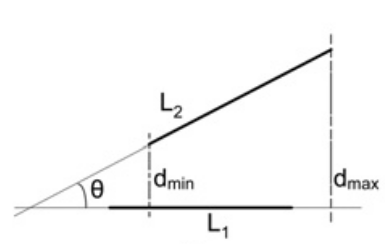
\includegraphics[width=0.4\textwidth]{./images/PGH_geo}}~~
\subfloat[The pairwise geometric histogram ]{\label{fig:example_2}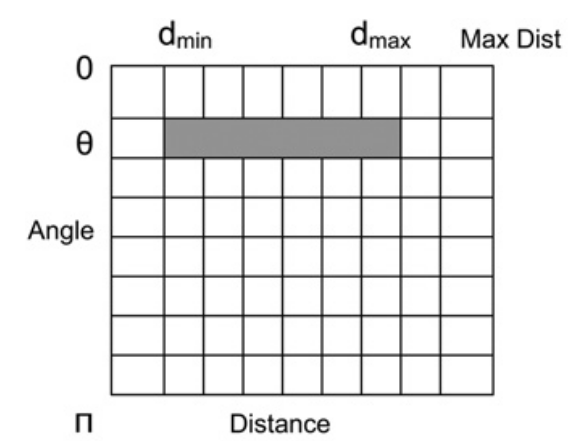
\includegraphics[width=0.4\textwidth]{./images/PGH}}
\caption{The geometric features and the PGH}
\label{fig:figure_31}
\end{figure}
\\[0.3cm]The frequency of the geometric features is recorded as a two dimensional histogram with an angle axis (0 - $\pi$) and distance axis (range of perpendicular distance). The entries on PGH describe the geometric relationship between the reference line and the object lines. The blurring of entry along the axis regarding the true position and orientation of each object lines for reference line.
\\The full object representation is constructed by recording the PGH for each line within object. If the object is defined by n lines, the full shape representation will composed of n pairwise geometric histograms.\\
This method still good when we apply some variants on the image, such as translate or rotate the image because the angle and perpendicular distance between a pair of lines is invariant.
\subsection{Histogram matching}
\section{Probabilistic Hough Transform}































